%. Introduction
%  Adsorbate-Metal systems 
%      catalysts
%      devices
%      oxide formation
%    This dissertation
%      structure
%      dynamics
%      reconstruction
%      accurate treatment of electronic interactions and charge transfer effects
%    Organized
%      1: Intro
%      2: Methodology Development
%      3: Pt-CO 557
%      4: Pt/Pd-CO 557
%      5: 112/557/321/765
%      6: MM-FlucQ
%      7: Summary
%
%  Metal Systems:
%      Structure
%        bimetallic (alloys, layers, near surface alloys, etc.)
%      Dynamics
%    Adsorbate Interactions:
%      binding sites
%      patterning
%    Dynamics
%      diffusion
%      step-wandering
%    Reconstruction
%      refaceting
%      doubling
%      island formation

\chapter{INTRODUCTION}
\label{chap:intro}
%CHAP1
%Metal surfaces
%  motivation (catalysis, energy generation, biomedical applications)
%  electronic, optical properties (stable at extreme temperatures, pressures for the most part)
%  list off neat things metal surfaces have done (20 or so spread throughout first couple of paragraphs
% Tie into importance of adsorbate interactions
Metal surfaces and nanoparticles play a large role in many areas of chemistry,
including catalysis,\citep{Clemens-Burda:2005qa, Sambur:2014mi} energy
conversion,\citep{Sneed:2014fj, Han:2015qr} and biomedical
applications.\citep{Padmos:0qf, Nicklin:0ss} The differences in their displayed
facets and morphologies can play a significant role in their
activity,\citep{Chiu:2012ec, Stephens:2011bv} selectivity,\citep{Yi:0qq} and
stability.\citep{Zhang:2015ys, Zhang:2007uq} Bimetallic species and alloys
along with supported surfaces and supported nanoparticles allow for an even
greater design space for various mechanical\citep{Cao:2010gf, Huang:2012ul} and
catalytic properties.\citep{Han:2015qr, Yu:2012by, Kim:2013mi, Jenness:2013oj}  In
most practical applications the surface of the metal will be exposed to a
variety of atmospheric compositions leading to numerous species adsorbed on the
surface.  For certain metals, under oxygen-rich conditions, there is also the
possibility of oxide formation which can dramatically change the surface
properties of the material.\citep{Streitz:1994mw, Derouin:2015kx} The
interactions between metals and adsorbates adds an additional layer of
complexity when attempting to fully describe metal surfaces since the presence
of adsorbates will perturb the electronic structure of the metal surface. If
the perturbation is large enough, surface reconstruction may become favorable which can
change the displayed surface facet.\citep{Kim:2013mi, Tao:2010aa, Tao:2008aa}

This dissertation is intended to provide a fundamental picture for adsorbate
induced reconstruction on metal surfaces by examining the complex interactions
present in these systems, measuring the perturbed dynamics, and analyzing the
effect of different exposed facets by using Molecular Dynamics (MD) simulations
to capture the atomic mechanisms that lead to restructuring.


%In general, the structure of metal surfaces can be strongly perturbed by the
%presence of adsorbates. The extent of adsorbate coverage and the strength of
%adsorbate self-interactions can both drastically affect the predicted
%low-energy surface. If the preferred low-energy is modified and the kinetic
%barrier is not too large, surface reconstructions can result.  Since the
%efficacy of metal surfaces strongly depends on the exposed structure, having a
%detailed understanding of the mechanism of surface dynamics and restructuring
%as caused by adsorbates is of the utmost relevance. 

The organization of this dissertation is such that a brief overview of metallic
systems, adsorbate interactions, and adsorbate-induced reconstructions is
presented in Chapter 1.  The second chapter presents work on the surface
reconstructions of Pt (557) and Au (557) surfaces when exposed to carbon
monoxide (CO). In Chapter 3 the effect of CO adsorption on a Pt/Pd (557)
subsurface alloy is explored. The fourth chapter more fully examines the
effects of different facets (step-type and plateau length) as they affect the
CO-induced restructuring of platinum. Moving away from Pt-CO systems, Chapter 5
presents our development of the mm-FlucQ potential and its applications to
charge transfer and oxide formation on Pt surfaces. Finally, Chapter 6 contains
a summary of this work as well as proposals for future directions.
%The second chapter focuses on accurately modeling the metal-metal,
%metal-adsorbate, and adsorbate-adsorbate interactions, along with introducing
%the multiple-minima fluctuating charge (MM-flucQ) method as it relates to the
%electrostatic interactions present in the system. 

\section{Metals}
Making up more than half of the periodic table, metals are usually
characterized by their high electrical and thermal conductivity along with
their malleability and ductility. These properties arise from their unique
electronic structure which is in contrast to non-metal molecular species.
Unlike other chemical species which tend to only share valence electron density
with their nearest (bonded) neighbors, metals are able to freely share their
valence electrons throughout the material.  This ``sea of electrons'' can be
described using an extension of molecular orbital theory, where instead of only
have a few bonding and anti-bonding molecular orbitals at various energy
levels, there are enough atomic orbitals from the numerous metal atoms to form
{\em bands} of bonding and anti-bonding orbitals which are labeled as
``valence'' and ``conduction'' bands respectively. In metals, there is
essentially no energy barrier for an electron to move from the top of the
valence band to the conduction band which is one of the reasons metals tend to
have high electrical and thermal conductivities, as compared to ``insulators''
which typically have large energy gaps between their HOMO and the LUMO
orbitals.


With regards to catalytic activity, the metals in columns 9, 10, and 11 (Pt,
Pd, Rh, etc.) of the periodic table tend to be highly active for certain
catalytic processes. This phenomenon can be somewhat explained by the Sabatier
Principle. For catalysis to occur the binding strength between
adsorbates and surfaces needs to be balanced. If the adsorbate binds too
strongly, it will be difficult to remove and will likely poison or deactivate
the catalyst. If the adsorbate binds too weakly, there is likely a concomitant
increase in the difficulty of scission of the adsorbate which is likely needed
for the catalytic reaction to occur. Thus the metals in columns 9-11 tend to
form bonds that are ``just right''; however, just as different metals will have
non-equivalent interactions with adsorbates, the structure of a single metal
can also lead to different preferred binding sites and binding energies.


\subsection{Structure}
The local structure of metals is quite important as it directly affects the
electronic properties which in turn can modify the catalytic activity of the
metal. To help visualize the structure, we can model metal atoms as equally
sized small spheres. The highest packing density can be achieved with either an A-B-C
layer stacking which results in a face-centered cubic (FCC) crystal structure
or an A-B-A layer stacking which results in the hexagonal close-packed (HCP)
crystal structure. Both possibilities are displayed in Figure
\ref{fig:packing}. While the bulk properties of metals are well-characterized,
the majority of chemistry happens at the surfaces of metals which
are more complex. Specifically, while metals tend to have FCC or HCP packing,
depending on the termination or ``slicing'' of the crystal a variety of exposed
surface facets are possible.

\begin{figure}[p!]
  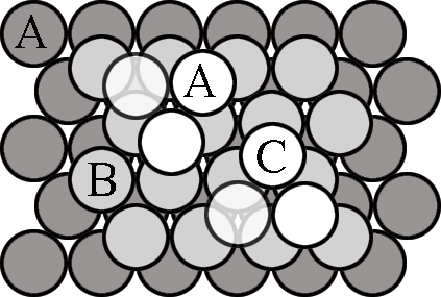
\includegraphics[width=\linewidth]{../figures/chap1/packing.pdf}
  \caption{Depiction of A-B-C and A-B-A layer stacking for FCC and HCP crystal
structures. The lowest layer of atoms compose an ``A'' layer, while the middle
atoms (gray) represent the ``B'' layer. The atoms in the third layer can sit
either directly above a hollow site in the middle layer and an atom in the
bottom layer leading to the A-B-A stacking and an HCP crystal structure, or sit
directly above two hollow sites leading to A-B-C stacking and an FCC crystal
structure.}
  \label{fig:packing}
\end{figure}

The three common low-energy (high-stability) facets for FCC and HCP
metals are shown in Figure \ref{fig:facets}. The facet labels, (100),
(110), and (111) represent the Miller indices of these surfaces and provide a
prescription for ``slicing'' a bulk crystal to obtain that surface. For many
metal surfaces, and for platinum and palladium in particular, the surface energy of the
(111) facet is the lowest while a higher-index,
{\em i.e.} rougher, surface will be more energetically expensive than the (111) facet.

\begin{figure}[p!]
  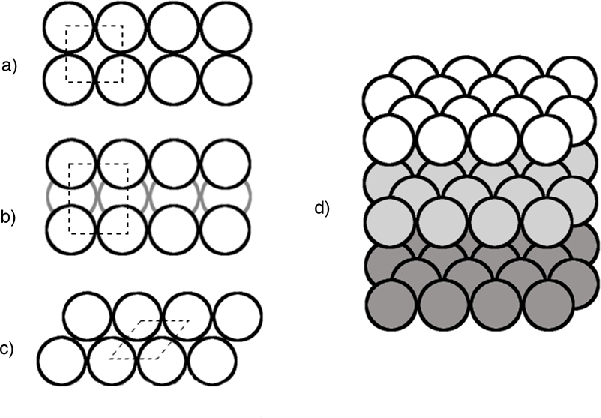
\includegraphics[width=\linewidth]{../figures/chap1/facets.pdf}
  \caption{On the left are displayed face-down views of common low-index facets
of metals (a) (100), (b) (110), and (c) (111). The dotted lines represent a
repeatable crystal unit on each facet. The light gray coloring in (b) is
illustrating the placement of that row of atoms behind the top and bottom row.
Facet (d) displays a (112) step edge. The darker shading represents separate
terraces that are displaced by one atomic height.}
\label{fig:facets}
\end{figure}

However, the presence of kinetic barriers coupled with the relatively large
size of metal surfaces leads to step-edges, one of the most commonly observed
structural defects.  These are highlighted in Figure \ref{fig:facets}.d.  The
(111) motif is still present; however, there are single atom height
displacements between plateaus. Due to their under-coordination, these edge
atoms will interact differently, often more strongly, with adsorbates,
potentially making those sites catalytically active.

There are other relatively common surface atoms that are under-coordinated on
metal surfaces and are often labeled as either kink atoms, describing an atom
that is at the vertex of two intersecting edges, or adatoms, which are free
atoms sitting on an otherwise flat surface. These atoms, because of their
under-coordination, are promising candidates for enhanced catalytic activity,
and designers of industrial catalysts attempt to increase the density of these
atoms.  Nanoparticles and nanospheres, have large surface curvature, and
exhibit a greater density of edge atoms, kink atoms, and adatoms, making them
of significant industrial interest.  Periodic surfaces that contain a large
density of edge and kink atoms can be constructed by ``slicing'' along certain
Miller indices.

\subsubsection{Bimetallic and supported systems}
In addition to the effect that local structure has on the electronic properties
of metals, the introduction of other metals through alloying or the presence of
non-metallic  supports that can donate or withdraw electron density will also
affect the properties and adsorbate binding behavior of the metal. The ability
to tune these deviations is of much interest and significant research has been
directed at examining various bimetallic species, including heterogeneous
alloys,\citep{Stamenkovic:2007kk, Yu:2013fr} core-shell
nanoparticles,\citep{Huang:2012ul, Tao:2008aa, Wang:2015qb} and near-surface
alloys\citep{Stephens:2011bv, Jan-Knudsen:2007fe} in order to design more effective
catalysts.  Figure \ref{fig:bimetallic} shows a number of ideal examples of
these types of systems. While synthesizing these systems can be challenging,
the ability to specifically tune the catalysts for certain reactions,
resistance to poisoning\citep{Yu:2013fr, Sharma:0ly}, and cheaper
costs\citep{Li:0hl, Zhao:0qf}, etc. provides a strong impetus for the
characterization of these materials.

\begin{figure}[p!]
  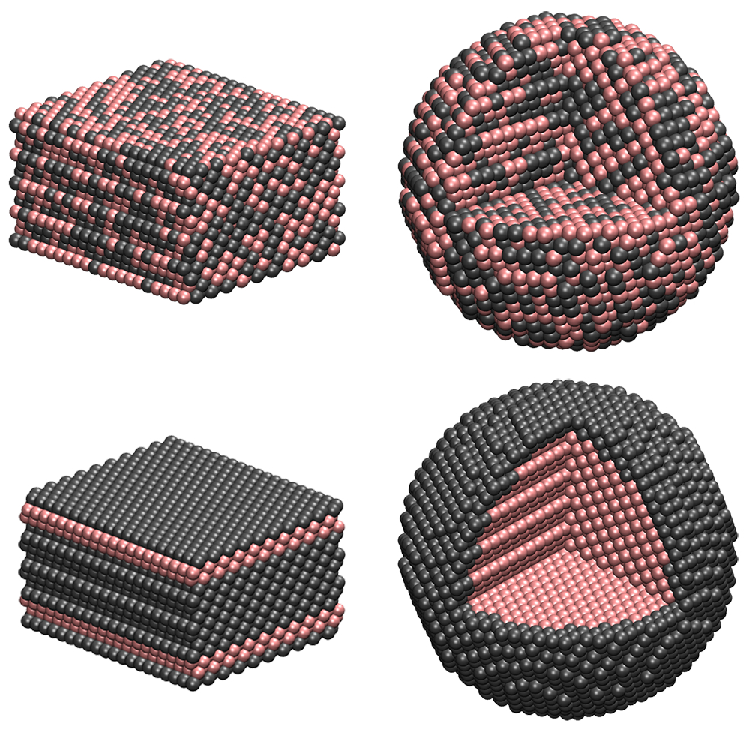
\includegraphics[width=\linewidth]{../figures/chap1/bimetallic.pdf}
\caption{The top two systems are Pt\textsubscript{0.5}Pd\textsubscript{0.5}
homogeneous alloys (Pt are shown in gray and Pd in pink), with the left
representing a (111) surface and the right image depicting a nanosphere with a
radius of 30~\AA. The bottom left image displays a near-surface alloy with two
layers of Pd sandwiched between layers of Pt while the right image shows a
core-shell nanosphere with a small section cut away to allow the thickness of
the shell to be seen.}
\label{fig:bimetallic} 
\end{figure}

\subsection{Dynamics}
Metal self-interactions are strong enough so that at room temperature minimal
movement of the metal atoms is observed. This is particularly true for
low-index facets since these surfaces tend to exist in relatively deep local
minima on the potential energy surface. However, these systems are also less
useful for applications due to that same stability leading to a general
weakening of the interactions between the metal surface and adsorbates.  Many
industrial processes make use of high-index or roughened nanoparticles, taking
advantage of their larger number of under- \& over-coordinated surface atoms,
since these atoms are often more active for catalytic
processes.\citep{Calle-Vallejo:2015qq, Stephens:2011bv} The increased density
of edge and kink atoms creates additional binding possibilities on the surface
and can also lead to easier adatom formation and surface mobility.
Additionally, the presence of adsorbates can also strongly affect the dynamics
of a metal surface because of the potential for strong interactions (primarily
repulsive) between adsorbates, which can effectively weaken the metal-metal
binding and allow for easier adatom formation.\citep{Tao:2010aa, Eren:2016qt}


\subsubsection{Diffusion \& step wandering}
Barring macroscopic perturbations and the resultant large-scale modification of
a metal surface, {\em i.e.} ablation, mechanical-cleaving, etc. all movement on
surfaces ultimately involves the movement of adatoms. The two primary modes of
adatom motion can be distinguished by: 1) the adatoms either moving
independently, defined here as diffusion, or 2) in a concerted fashion, defined
here as step-wandering. While it is helpful to divide these as two distinct
modes, they are perhaps better thought of as two sides of the same coin.
Independent adatom movement is statistically more likely to be observed as it
only requires one surface atom to be ejected from a stable edge or terrace or
upwards from a surface.  Since the strength of metallic bonding is proportional
to the number of nearest neighbors, once an adatom is created and is seated on
the surface, there is often only a minimal energy barrier for the adatom to
continue moving around on the surface.

The second main type of movement involves cooperative adatom diffusion and is
better described as entire step-edges ``wandering'' on the surface. This
wandering is ultimately a collection of ejection of adatoms from step-edges
followed by their re-admittance to the step-edge at a different position. It is
possible to observe the large-scale step-wandering by following these
individual events. Understanding the dynamics of step-edge wandering is
necessary to characterize reconstruction events, since they tend to involve the
appearance or disappearance of step-edges and their presence tends to raise the
surface energy of a system while lowering its stability.

\section{Adsorbate Interactions on Metal Surfaces}
The majority of applications involving metals depend on the metal
surface providing a favorable environment for some other reaction to occur,
whether that be oxidation of CO, production of \ce{H2} through a
water-gas-shift reaction, or some other mechanism that involves molecules
adsorbing to a surface. Having an accurate understanding of how adsorbates
interact with metal surfaces is thus of great importance when attempting
to design more effective catalysts.

\subsection{Binding sites}
While bulk metals are well described by their high symmetry and formation of
electronic bands, the introduction of surfaces break that symmetry. This results in the re-hybridization of
metallic orbitals upon approach of adsorbates. While the idea is not
exact, thinking of surface metal atoms as possessing atomic {\em s, p, } and {\em d}
orbitals available for bonding as in regular molecular orbital theory can be
helpful. On a (111) surface there are three primary binding sites, the 1-fold
(atop), 2-fold (bridge), and 3-fold (hollow) sites, which are highlighted in
Figure \ref{fig:binding}. 

\begin{figure}[p!]
  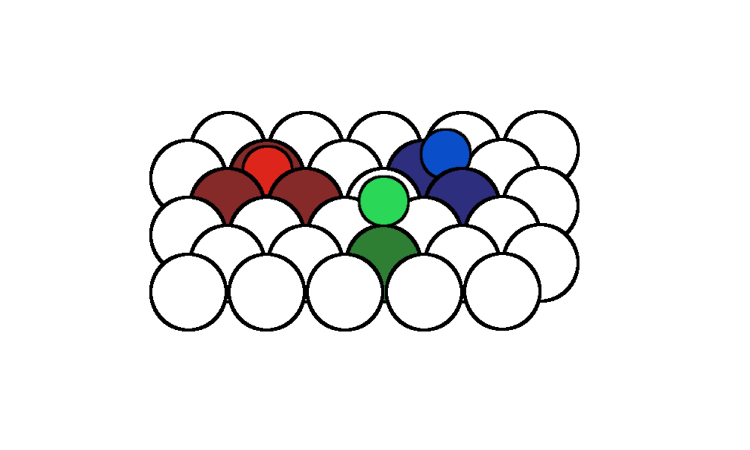
\includegraphics[width=\linewidth]{../figures/chap1/binding.pdf}
  \caption{The atop (green), bridge (blue), and three-fold hollow (red)
adsorption sites are the three most common binding sites for small molecules on
low-index FCC and HCP surfaces. The extent of the orbital overlap between the surface and the adsorbate coupled with the coverage all affect the preferred binding site.}
\label{fig:binding}
\end{figure}

As an illustrative example, carbon monoxide on platinum (111) has been studied
extensively\citep{Ertl:1977cg, Kelemen:1979ad, Yeo:1997th, Wong:1991ta,
Feibelman:2001qa, Deshlahra:2009wu, Deshlahra:2012aa} and is often used as a
model for molecular adsorption on metal surfaces.  Hoffman {\em et al.},
utilizing the extended H\"uckel method,\citep{Wong:1991ta} was able to
calculate the overlap population between the CO and Pt orbitals and how they
changed depending on the CO  binding site.  When CO was placed in the atop
position, the CO $5\sigma$ (HOMO) orbital only interacted with 3 of Pt's
frontier orbitals, specifically the $6s$, $5p_z$, and $3d_{z^2}$. However, when
they placed CO into the 3-fold hollow site, all nine surface bands showed at
least some overlap with CO's 5$\sigma$ orbital. While this type of analysis has
become more mainstream, predictions of preferred binding sites are still
difficult, especially since they are often coverage-dependent.

\subsection{Coverage dependence}
While there might be one preferred binding site for a single adsorbate on a
metal surface, the presence of strong adsorbate-adsorbate interactions can lead
to deviations from expected behavior. Again looking to CO on Pt (111), at low
coverages ($<$ 0.25 monolayer (ML)), CO has been observed to bind primarily to
atop sites.\citep{Kelemen:1979ad, Feibelman:2001qa} As the coverage increases
however, adsorbate-adsorbate repulsion causes the preferred binding to change
to a mix of atop and bridge sites.\citep{Deshlahra:2012aa} Typically,
adsorbate-adsorbate interactions are repulsive which results in weaker surface
binding and can induce strain in the metal surface resulting in lower potential
energy barriers for surface reconstruction.


For certain molecules, adsorbate-adsorbate interactions can be cooperative.
Schneider {\em et al.} performed DFT calculations of CO on Pt (111) at 0.5 ML
coverage and observed that the preferred binding of the adsorbate was a mix of
atop and bridge sites.\citep{Deshlahra:2012aa} This mixed configuration was due
to non-equivalent $2\pi^*$ back-donation from the platinum to the CO which
created favorable dipole-dipole interactions between the atop bound CO and the
bridge bound CO.  Specifically, carbon monoxide bound to an atop site
experienced less back-donation and was calculated to have a positive dipole
moment while the carbon monoxide bound to the neighboring bridge site
experienced a greater amount of electron donation and exhibited a negative
dipole moment.


\subsubsection{Adsorbate patterning}
%Image of particles adsorbed on the surface
In addition to the adsorbate-metal interactions, there are also complex
interactions between adsorbates that can lead to large-scale patterning observable
with XPS (X-Ray Photo-electron Spectroscopy), LEED (Low Energy
Electron Diffraction), and other experimental techniques. These
adsorbate-adsorbate interactions cause the preferred binding sites to be
coverage dependent, since the presence and amount of bound adsorbates
affects the energy levels of the surface and in particular the energies at the
different binding sites.

Thus, at distinct coverages, different adsorbate patterns are observed. For example,
\ce{CO} on \ce{Pd} at surface coverage ($\theta$) of $1/3$ ML tends to be arranged in a
$(\sqrt{3}\times\sqrt{3})\textrm{R}30$\textsuperscript{o} pattern. However, raising the coverage
to a half-monolayer, $\theta = 1/2$, causes the experimentally observed
patterning to change to a c$(4\times2)$ pattern. If the coverage is further
increased to three-quarters monolayer, $\theta = 3/4$, the preferred pattern is
a $(2\times2)$ pattern.\citep{Guo:1989aa} These patterns are all shown in
Figure \ref{fig:patterns}.

\begin{figure}[p!]
\centering
  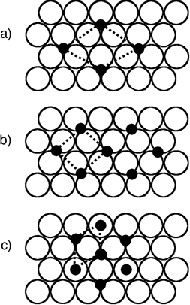
\includegraphics[width=0.5\linewidth]{../figures/chap1/pattern.pdf}
  \caption{Adsorbate patterns of CO (black dots) on Pd (111) (white spheres), (a)
$(\sqrt{3}\times\sqrt{3})\textrm{R}30^o$, (b) c$(4\times2)$, (c) $(2\times2)$.}
\label{fig:patterns}
\end{figure}

A good model of the adsorbate and adsorbate-metal interactions should be able
to capture some of these different patterns; however, capturing every possible
arrangement is beyond the scope of most non-quantum mechanical treatments.

\section{Surface reconstructions}
% Studies done on clean metal surfaces tend to suffer from pressure and temperature gaps
% high pressure xps, stm, spin echo helium bombardment provide some ways to mimic the environment of industrial catalysts
% Difficult to determine mechanisms because of time and spacial resolution
% DFT good at calculating relative energies for small systems, but the size of these reconstructions makes calculations expensive
% mol dyn. allows us to explore the interactions that lead to adsorbate-induced reconstructions

Metal surfaces often remain stable even when the environment is perturbed,
although the presence of adsorbates can sufficiently modify the potential
energy surface of the metal such that a new facet is energetically favored.
This situation might even be commonplace, but altering the potential energy
surface does not ensure that a reconstruction will take place. The system must
also be able to overcome any energy barriers that would trap the surface in a
local minima.  For systems that are started far from a low surface energy
state, ({\em i.e.} nanoparticles and roughened surfaces) the introduction of
adsorbates will likely lead to a restructuring to a lower-energy structure. 

The time and length scales of these reconstruction processes can vary widely
depending on the specific system and conditions and have been estimated to occur
over times as fast as nanoseconds or as slowly as minutes\citep{Tao:2010aa,
Eren:2016qt} While current experimental techniques are able to observe and
identify the reconstructions, they are often unable to identify the 
mechanisms of reconstructions which could prove crucial in designing better
catalysts.

\subsection{Refaceting}
Refaceting is a more specific term used to describe surface reconstructions
that proceed from one well-defined facet to another.  If a bulk crystal is cut
at too large of an angle away from a low-energy surface, there will be a strong
driving force to re-facet. Barring large kinetic barriers that keep certain
facets as metastable states, a surface facet will reconstruct so long as the
surface normal vector $\hat{n}_0$ of the facet is conserved and the overall
tension $\gamma$ is reduced as shown in the relations derived by
Herring\citep{Herring:1951ta}, where $A_i$ is the area of the surface of
orientation $\hat{n}_i$.

\begin{equation}
A_0\hat{n}_0 = A_a\hat{n}_a + A_b\hat{n}_b
\end{equation}
\begin{equation}
A_0\gamma(\hat{n}_0) > A_a\gamma(\hat{n}_a) + A_b\gamma(\hat{n}_b)
\end{equation}

This reconstruction should only occur in the forward direction and while an
increased temperature is often sufficient for overcoming the energy barrier,
the presence of adsorbates has also been seen to cause
reconstructions.\citep{Eren:2016qt, Williams:1994aa, Jeong:1999ev} 

\subsubsection{Step-Edge doubling}
Work by Tao {\it et al.} on a \ce{Pt} (557) surface observed a reversible
reconstruction event that was directly dependent on the presence or absence of
\ce{CO} in the system.\citep{Tao:2011aa} When \ce{CO} was introduced to the
system the step-edges doubled in height, but upon removal of the \ce{CO} the original
(557) motif was recovered. This reversible reconstruction strongly implies that
the presence of \ce{CO} temporarily modified the potential energy surface to
prefer a new ground state structure; however, the exact mechanism of this
reconstruction was not deduced at the time. 

\subsection{Island formation and sintering}
Since catalytic reactions typically only occur at the surface of metals,
significant research has been devoted to increasing the surface area to volume
ratio of metal catalysts, either through catalyst supports, high-index
nanostructures, or bimetallic near-surface alloys. While these systems are
typically stable at low temperatures and pressures, significant perturbations
can lead to what is effectively sintering or island-formation of one of the
metals on the surface.  The interplay of surface energies and adsorbate
interactions on two or more metal surfaces allows for the creation of
highly tuned catalysts.

\section{Modeling metals}
The modeling of molecular systems, and metals in particular, requires an
accurate description of the particles present in the system and most
importantly the interactions they have with each other. Depending on what
properties are being searched for, the accuracy and the associated expense of
these interactions can vary drastically. For instance, modeling catalytically
activated chemical reactions on a metal surface with the intent of mapping
reaction pathways requires a higher level of theory when compared to modeling
large-scale reconstructions of metals as a result of high temperature and
pressure.

Generally, simulations can be broken up between two main classes, those that
require an accurate treatment of electron movement and transfer and those that
can suffice with a minimal amount of electron treatment.  Metals are at an
interesting junction between these two domains as their electronic nature does
play an important role in their interactions with adsorbates; however,
capturing the reconstructions observed on metal surfaces requires large system
sizes that can not currently be treated at such a high level of theory. Thus,
for the systems examined in this dissertation, the metal-metal and metal-CO
interactions will be represented with a simpler model so that the size of the
systems and length of the simulations can be expanded to capture reconstruction
events.

\subsection{Molecular Dynamics}
In constrast to Density Functional Theory and other methods that attempt to
solve the electronic wavefunctions within a molecular system, most
implementations of molecular dynamics sacrifice this portion of the molecular
description in order to gain the ability to model larger systems ($>$1000s of
atoms) for longer times ($>$1e6 fs). At a minimum, a molecular dynamics
implementation requires knowledge of the positions, $\mathbf{r}$, and
velocities, $\mathbf{v}$, of all $N$ particles in the system along with a
complete description of the cross-interactions between all pairs of particles.
The accumulation of the different interaction potentials is also known as a
``forcefield''. With this knowledge and a suitably chosen timestep ($\sim$ 1-2
fs), the system can be evolved through time by integrating Newton's equations
of motion. A general approach for the procedure is shown below.

%list
\begin{enumerate}
\item Given initial $\mathbf{r}$ and $\mathbf{v}$, set the time $t=0$ and
$\Delta t$ to something suitably short.

\item Move atoms based on current positions and velocities.

\begin{equation*}
r_i(t + \Delta t) = r_i(t) + v_i(t)*\Delta t + a_i(t)*\Delta t^2 + ...
\end{equation*}

\item Update velocities.
\begin{equation*}
v_i(t + \Delta t) = v_i(t) + a_i(t)*\Delta t^2 + ...
\end{equation*}

\item Calculate forces from updated positions.
\begin{equation*}
F_i = -\nabla V(\mathbf{r})
\end{equation*}

\item Correct positions, velocities, etc. with new force information.
\item Apply conditions (thermostats, barostats, etc.).
\item Measure properties of interest.
\item Repeat steps 2-8 until some pre-establishted condition is met.
\end{enumerate}

The specific implementation of position and velocity integration as briefly
mentioned in numbers 2 and 3 can vary and numerous algorithms exist including
verlet\citep{Verlet:1967aa} and velocity-verlet
integration.\citep{Dullweber:1997aa} The conditions mentioned in number 6 are
in reference to methods that can ensure that the system is maintained at a
given temperature or pressure and while important, go beyond our introduction
to molecular dynamics, but further resources can be found in References
\citep{Hoover:1985aa, Melchionna:1993aa, Leach:2001aa}.

While all of the above mentioned steps are important in some way, number 4, the
calculation of forces is potentially the most important as it deals with all of
the interactions in the system. As the forces are obtained from the interaction
potential, a brief overview of metal-metal and metal-CO potentials
will conclude our introduction to molecular dynamics simulations.

\subsubsection{Metal-Metal interaction potentials}
Many of the potentials used for modeling transition metals are based
on a non-pairwise additive functional of the local electron
density. The embedded atom method (EAM) is perhaps the best known of
these
methods,\citep{Foiles:1986ky, Daw:1984aq, Johnson:1989yr, Daw:1989ci, Plimpton:1993qi, Voter:1995ax, Lu:1997fv, Alemany:1998fp}
but other models like the Finnis-Sinclair\citep{Finnis:1984hl, Sutton:1990rr} and
the quantum-corrected Sutton-Chen method\citep{Goddard:1998qsc, Qi:1999dn} have simpler
parameter sets. The glue model of Ercolessi {\it et
  al}.\citep{Ercolessi:1988uo} is among the fastest of these density
functional approaches. In all of these models, atoms are treated as a
positively charged core with a radially-decaying valence electron
distribution. To calculate the energy for embedding the core at a
particular location, the electron density due to the valence electrons
at all of the other atomic sites is computed at atom $i$'s location,
\begin{equation}
\bar{\rho}_i = \sum_{j\neq i} \rho_j(r_{ij})
\end{equation}
Here, $\rho_j(r_{ij})$ is the function that describes the distance
dependence of the valence electron distribution of atom $j$. The
contribution to the potential that comes from placing atom $i$ at that
location is then
\begin{equation}
V_i =  F[ \bar{\rho}_i ]  + \sum_{j \neq i} \phi_{ij}(r_{ij})
\end{equation}
where $F[ \bar{\rho}_i ]$ is an energy embedding functional, and
$\phi_{ij}(r_{ij})$ is a pairwise term that is meant to represent the
repulsive overlap of the two positively charged cores.  

% The {\it modified} embedded atom method (MEAM) adds angular terms to
% the electron density functions and an angular screening factor to the
% pairwise interaction between two
% atoms.\citep{BASKES:1994fk,Lee:2000vn,Thijsse:2002ly,Timonova:2011ve}
% MEAM has become widely used to simulate systems in which angular
% interactions are important (e.g. silicon,\citep{Timonova:2011ve} bcc
% metals,\citep{Lee:2001qf} and also interfaces.\citep{Beurden:2002ys})
% MEAM presents significant additional computational costs, however.

The EAM, Finnis-Sinclair, and the Quantum Sutton-Chen (QSC) potentials
have all been widely used by the materials simulation community for
simulations of bulk and nanoparticle
properties,\citep{Chui:2003fk, Wang:2005qy, Medasani:2007uq, Mishin:1999ew}
melting,\citep{Belonoshko:2000jk, Sankaranarayanan:2006ye, Sankaranarayanan:2005bh}
fracture,\citep{Shastry:1996qg, Shastry:1998dx, Mishin:2001qt} crack
propagation,\citep{Becquart:1993sr, Rifkin:1992ug} and alloying
dynamics.\citep{Shibata:2002hh, Mishin:2002if, Zope:2003ai, Mishin:2005vc}
One of EAM's strengths is its sensitivity to small changes in
structure. This is due to the inclusion of up to the third nearest
neighbor interactions during fitting of the parameters.\citep{Voter:1995ax}
In comparison, the glue model of Ercolessi {\it et
  al}.\citep{Ercolessi:1988uo} was only parameterized to include
nearest-neighbor interactions. EAM is thus a suitable choice for systems
where the bulk properties are of secondary importance to low-index
surface structures. Additionally, the similarity of EAM's functional
treatment of the embedding energy to standard density functional
theory (DFT) makes fitting DFT-derived cross potentials with
adsorbates somewhat easier.

\subsubsection{Lennard Jones \& Morse potentials}
Accurately modeling the charge-transfer associated with bond formation between
adsorbates and metal surfaces requires either a reactive forcefield or a
quantum mechanical treatment of the system, both of which are too computationally expensive
for the size of the simulations explored in this dissertation. Assuming minimal effects
from charge transfer, which to first order is satisfactory, formation
of a metal-adsorbate bond can be sufficiently represented by a combination of
Lennard Jones and Morse potentials, see equations \ref{eq:lj} and \ref{eq:mp}.

\begin{equation}
V(r) = 4\epsilon\bigg(\bigg(\frac{\sigma}{r}\bigg)^{12} - \bigg(\frac{\sigma}{r}\bigg)^6\bigg)
\label{eq:lj}
\end{equation}

\begin{equation}
V(r) = D_e(1-e^{-\gamma(r-r_e)})^2
\label{eq:mp}
\end{equation}


Both potentials describe the energy of two particles as they approach each
other. The Lennard Jones potential is parameterized by two variables, $\sigma$,
which describes the ``size'' of the atom, and $\epsilon$, which scales the
strength of the interaction, while the Morse potential is composed of three
variables, $D_e$, an energy scaling term, $r_e$, the minimum energy separation
distance and, $\gamma$, a knob on which to tune the tightness of the well.

The potentials, along with their sum are displayed in Figure
\ref{fig:potentials}. The Lennard Jones potential describes the Pt-C
interaction and is highlighted in orange. This potential is composed of two
pieces, a $\frac{1}{r^{12}}$ term that is responsible for the large repulsive
wall at short distances and a $\frac{1}{r^{6}}$ term that is attractive and has
its basis in instantaneous dipole-dipole interactions.


\begin{figure}
\centering
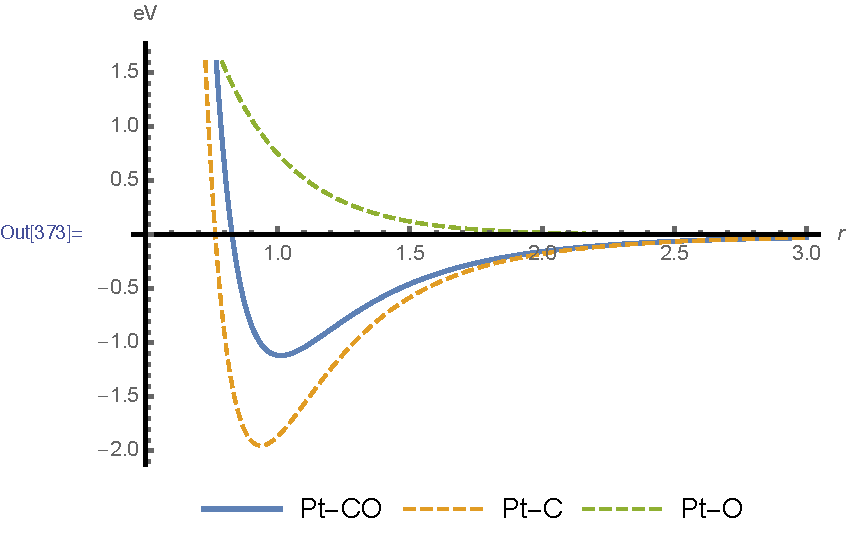
\includegraphics[width=\linewidth]{../figures/chap1/bindingEnergy.pdf}
\caption{These potential curves represent one of the parameterizations for the Pt-CO
interaction split into its component Lennard-Jones and Morse potential pieces.
The solid blue curve represents the Pt-CO potential provided in Chapter
\ref{chap:island} while the dashed orange curve represents the
Lennard-Jones interaction between Pt and C. The repulsive Pt-O interaction is
represented by the dashed green curve.}
\label{fig:potentials}
\end{figure}

The \ce{Pt\bond{-}O} interaction was initially represented with a Morse
potential for the work performed in Chapter \ref{chap:PtAu} but was changed to
the form below because of artificial oxygen first binding that was observed
infrequently on the highest coverage systems. This modification ensures that
the \ce{Pt\bond{-}O} bond is purely repulsive so that only \ce{Pt\bond{-}C}
binding is observed.

\begin{equation}
V(r) = D_e(e^{-2\gamma(r-r_e)})
\end{equation}

The only interactions not yet mentioned are the CO self
interactions which are being used unchanged from Karplus and
Straub.\citep{Straub:1991no} As the role of the strong CO-CO quadrupole
interaction is quite important in the reconstruction of some metal
systems,\citep{Tao:2010aa, Eren:2016qt} an in-depth examination of this model
is provided in Chapter \ref{chap:PtAu}.

